    \begin{frame}{Thuật toán tiến hóa}
		\begin{figure}
            \centering
                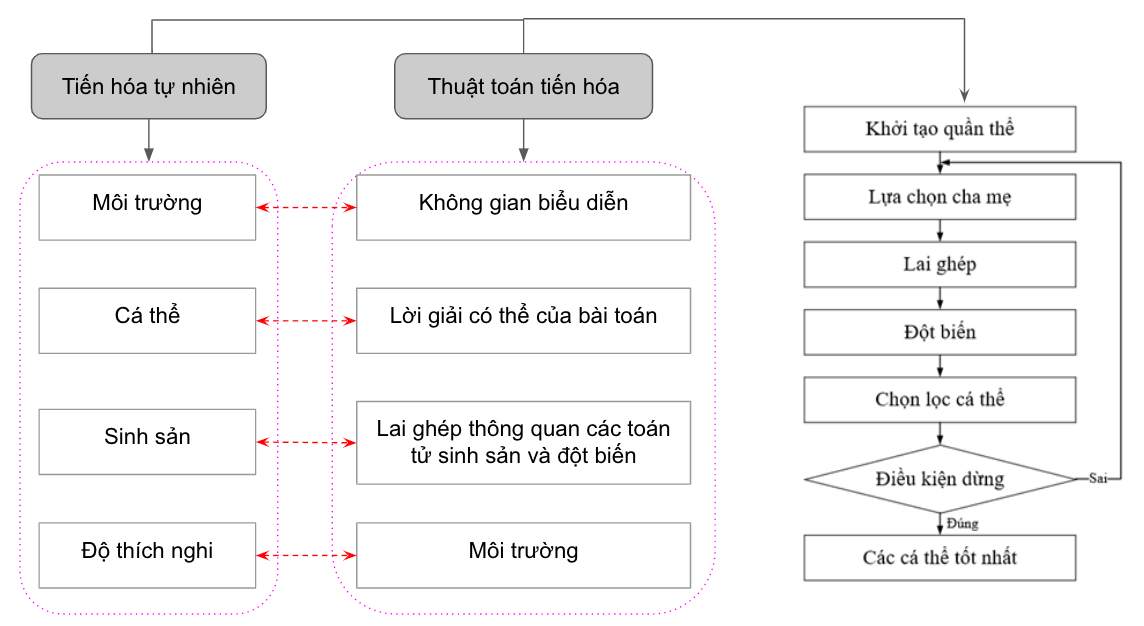
\includegraphics[width=1.0\textwidth]{images/ea_.png}
            \caption{Tổng quan thuật toán tiến hóa}
            \label{fig:mfo}
        \end{figure}
	\end{frame}
	
	\begin{frame}{Tối ưu hóa đa yếu tố (MFO)}
	    \begin{columns}
	    \column{0.6\linewidth}
		\begin{itemize}
	    	\begin{block}{Khái quát MFO}
        		\begin{itemize}
                \item Cho K tác vụ tối ưu $T_1, ..., T_k$
                \item Tác vụ thứ $i$ ký hiệu là $T_i$ có hàm mục tiêu vô hướng: $f_i: X_i \rightarrow \mathbf{R}$
                \item Các cá thể được mã hóa trong không gian tìm kiếm chung: $X_1, X_2, ..., X_k$
                \item Mỗi cá thể được giải mã dựa theo tác vụ đánh giá.
                \end{itemize}
			\end{block}
			\begin{block}{Mục tiêu}
			    Tối ưu K tác vụ đồng thời:
			    \begin{center}
                    \centering
                    ${x_1, x_2, ..., x_k} = \min \{f_1(x), f_2(x), ..., f_k(x)\}$
                \end{center}
        		\begin{itemize}
                \item $x_i$ là lời giải phù hợp trong tập $X_i$
                \item $f_i$ được coi yếu tố (factor) ảnh hưởng đến quá trình tiến hóa
                \end{itemize}
			\end{block}
		\end{itemize}
		\column {0.35\linewidth}
		\begin{figure}
            \centering
                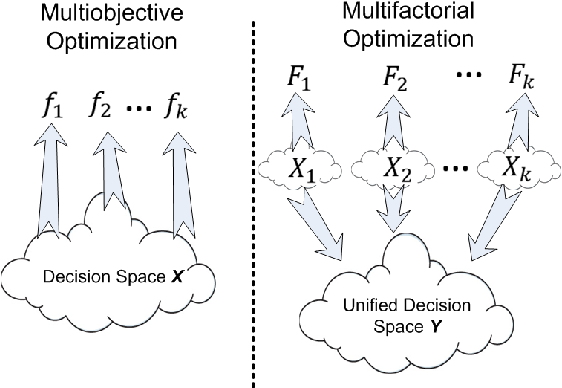
\includegraphics[width=1.0\textwidth]{images/mfo.png}
            \caption{So sánh tối ưu hóa đa yếu tố và tối ưu hóa đa mục tiêu (MOO và MFO)}
            \label{fig:mfo}
        \end{figure}
		\end{columns}
	\end{frame}
	
    \begin{frame}{Tiến hóa đa nhiệm - MFEA-I}
		\begin{figure}[h!]
            \centering
            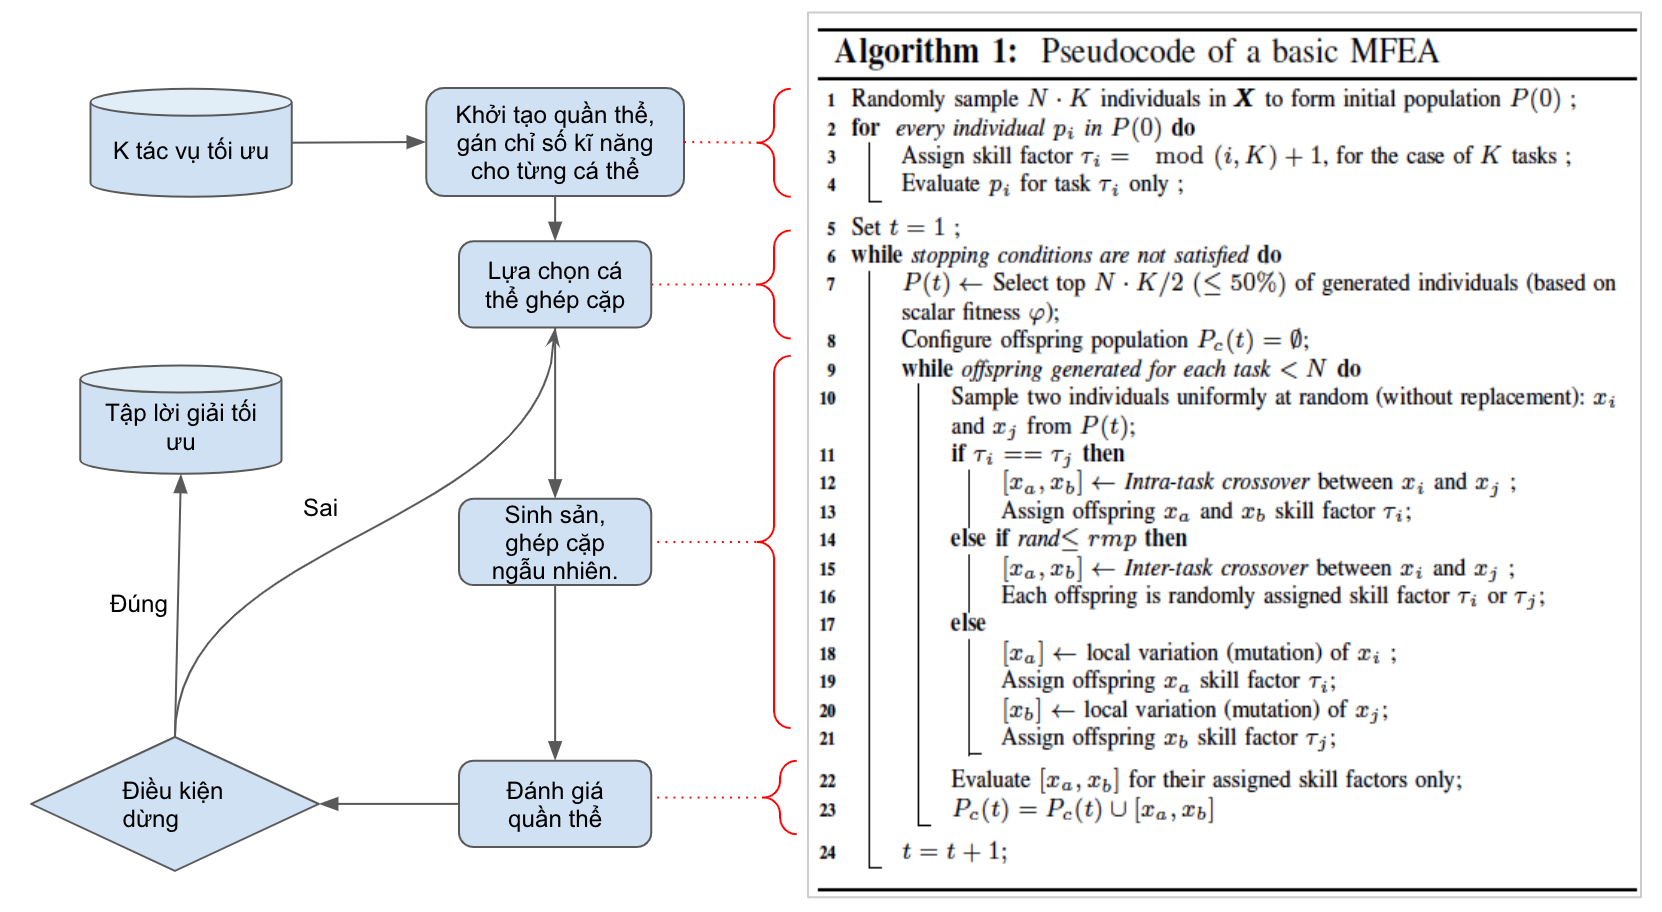
\includegraphics[width=1.0\linewidth]{images/mfeai_vi.png}
            \caption{\small{Khái quát MFEA-I}}
            \label{fig:mfeaii}
        \end{figure}
	\end{frame}
	
	\begin{frame}{Mô hình hỗn hợp - Mixture Models}
	    \begin{columns}
	    \column{0.7\linewidth}
		\begin{itemize}
	    	\begin{block}{Mixture Models trong môi trường đa nhiệm}
        		\begin{itemize}
        		\setlength\itemsep{0.03em}
                \item \textbf{Mixture Models} là mô hình hỗn hợp phân phối xác suất đại diện cho các quần thể con trong tổng thể.
                \item Cho $K$ tác vụ với $k \in \{1,2,...K\}$. tương ứng với mỗi tác vụ có quần thể con tại thế hệ thứ $t$ là $p^1(x,t), p^2(x,t),...., p^k(x,t)$.
                \end{itemize}
                \textcolor{blue}{Quần thể con cái sinh ra tại thế hệ thứ \textit{t}}:
                	\begin{equation}
                        q^k(x,t) = \alpha_k \cdot p^k(x,t) + \sum_{j \neq k} \alpha_j \cdot p^j(x,t)
                        \label{equa:mixture_distribution}
                    \end{equation}
                \begin{itemize}
                    \item Phân phối $q^k(x,t)$ là một hỗn hợp $K$ phân phối với hệ số hỗn hợp là $\alpha^{'}s$ với $\alpha_k + \sum_{j \neq k} \alpha_j = 1$ và $\alpha^{'}s >= 0$
                    \item Quá trình trao đổi tri thức giữa các tác vụ để tạo ra thế hệ con cái tốt hơn.
                \end{itemize}
                \Rightarrow Khi hai tác vụ hoàn toàn không bổ trợ cho nhau? \emph{negative transfer}
			\end{block}
		\end{itemize}
		\column{0.27\linewidth}
		\begin{figure}
            \centering
                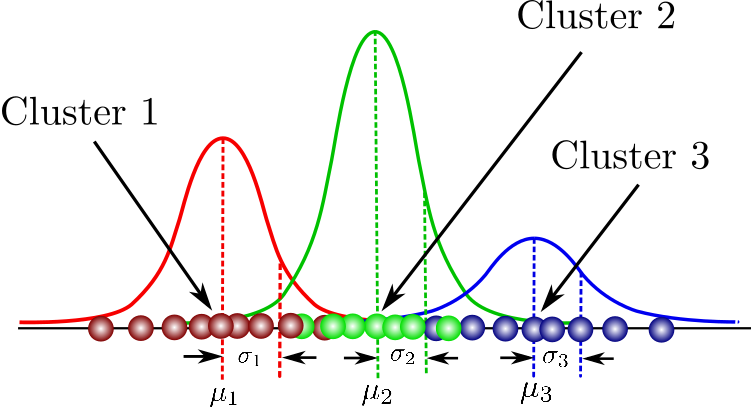
\includegraphics[width=1.0\textwidth]{images/mixture-prob.png}
                \caption{Hỗn hợp phân phối}\\
                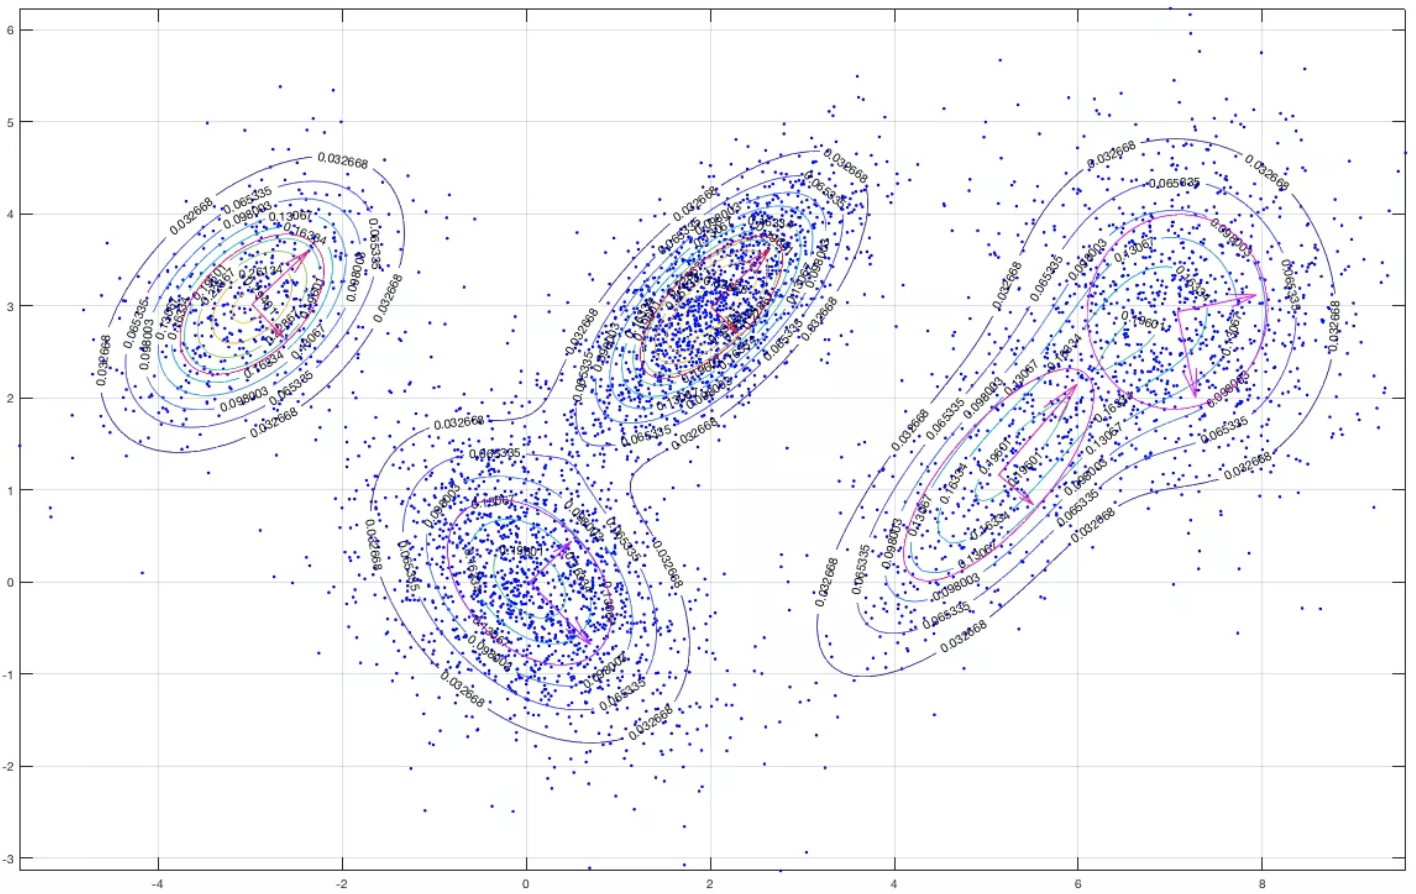
\includegraphics[width=1.0\textwidth]{images/mixture-model.png}
            \caption{Mô hình hỗn hợp quần thể}
            \label{fig:mixture-model}
        \end{figure}
		\end{columns}
	\end{frame}
	
	\begin{frame}{MFEA-I dưới góc độ xác suất}
		\begin{itemize}
	    	\begin{block}{Mô tả MFEA-I dưới thuật ngữ xác suất}
        		\begin{itemize}
        		\setlength\itemsep{0.03em}
                \item Tại thế hệ thứ $t$, $K$ tác vụ có quần thể chung $P_t$
                \item Tác vụ $k$ tại thế hệ thứ $t$ có quần thể con là $P_t^k$
                \item $P_t$ biểu diễn phân phối $p(x,t)$, thế hệ con cái của nó được biểu diễn $p_c(x,t)$
                \item $P_t^k$ biểu diễn phân phối $p^k(x,t)$, thế hệ con cái của nó được biểu diễn $p_c^k(x,t)$
                \end{itemize}
			\end{block}
			\begin{block}{Giả định}
                \begin{itemize}
                \setlength\itemsep{0.03em}
                \item Toán tử sinh sản là toán tử \textcolor{red}{parent-centric}
                \item $p_c(x,t) \approx p(x,t)$
                \end{itemize}
			\end{block}
			\begin{block}{Vấn đề}
			    \begin{itemize}
			    \item $p_c^k(x,t) \approx p^k(x,t)$?
                \item Mối quan hệ giữa $\mathbf{p_c^k(x,t)}$ với $p^j(x,t)$ $\mathbf{\forall j \neq k, j \in {1, ..., K}}$?
                \end{itemize}
			\end{block}
		\end{itemize}
	\end{frame}
	\begin{frame}{MFEA-I dưới góc độ xác suất}
		\begin{itemize}
	    	\begin{block}{Phân phối của thế hệ con cái}
                Thế hệ con cái là một hỗn hợp phân phối xác suất từ phân phối các cá thể của thế hệ cha mẹ.
                \begin{equation}
                p_c^k(x,t) = [1 - \frac{0.5 \cdot (K - 1) \cdot rmp}{K} ] \cdot p^k(x,t) + \sum_{j \neq k}\frac{0.5 \cdot rmp}{K} \cdot p^j(x,t). 
                \label{equa:mfea_offstring_distribution}
                \end{equation}
                % Trong đó $[1 - \frac{0.5 \cdot (K - 1) \cdot rmp}{K} ] $ và $\frac{0.5 \cdot rmp}{K}$ là các hệ số trao đổi. $rmp$ là hệ số \emph{giao phối ngẫu nhiên}.
			\end{block}
			\begin{block}{Giải pháp: Tối ưu sao cho $p_c^k(x,t)$ gần $p^k(x,t)$ nhất có thể}
                \begin{itemize}
                    \setlength\itemsep{0.03em}
                    \item Đơn giản: Đặt giá trị $\mathbf{rmp=0}$
                        \begin{itemize}
                            \item Sẽ không có sự trao đổi tri thức giữa các tác vụ.
                            \item Tuy nhiên không khai thác được mối quan hệ tiềm ẩn giữa các tác vụ. 
                        \end{itemize}
                    \item Phức tạp: Tối ưu $\mathbf{rmp}$ tùy thuộc vào mối quan hệ của từng cặp tác vụ
                        \begin{itemize}
                        \setlength\itemsep{0.03em}
                            \item Kiểm tra nếu quần thể của 2 tác vụ là \emph{"gần nhau"} thì mức độ trao đổi sẽ lớn và ngược lại.
                            \item Phụ thuộc vào phân phối của quần thể con tương ứng với tác vụ: $p^k(x,t)$ và $p^j(x,t)$ $\forall k,j \in {1,...,K}$ và $k \neq j$.
                        \end{itemize}
                \end{itemize}
			\end{block}
		\end{itemize}
	\end{frame}
% 	\begin{frame}{MFEA-I dưới góc độ xác suất}
% 		\begin{itemize}
% 		    \begin{block}{Vấn đề: Trong trường hợp các tác vụ không bổ trợ cho nhau}
%                 \begin{itemize}
%                 \setlength\itemsep{0.03em}
%                 \item Thế hệ con cái sinh ra sẽ chủ yếu nhận thông tin từ tác vụ bố mẹ của chúng.
%                 \item Từ công thức (\ref{equa:mfea_offstring_distribution}) ta suy ra cần tối ưu sao cho $p_c^k(x,t) \approx p^k(x,t)$.
%                 \end{itemize}
%                 \textbf{$\Rightarrow$ Cần phải điều chỉnh tham số $rmp$ sao cho $p_c^k(x,t)$ gần $p^k(x,t)$ nhất có thể.}
% 			\end{block}
% 	    	\begin{block}{Giải pháp}
%                 \begin{itemize}
%                     \setlength\itemsep{0.03em}
%                     \item Đơn giản: Đặt giá trị $\mathbf{rmp=0}$.
%                         \begin{itemize}
%                             \item Sẽ không có sự trao đổi tri thức giữa các tác vụ.
%                             \item Tuy nhiên không khai thác được mối quan hệ tiềm ẩn giữa các tác vụ. 
%                         \end{itemize}
%                     \item Phức tạp: Tối ưu $\mathbf{rmp}$ tùy thuộc vào mối quan hệ của từng cặp tác vụ
%                         \begin{itemize}
%                         \setlength\itemsep{0.03em}
%                             \item Kiểm tra nếu 2 tác vụ là \emph{"gần nhau"} thì mức độ trao đổi sẽ lớn và ngược lại.
%                             \item Phụ thuộc vào phân phối của quần thể con tương ứng với tác vụ: $p^k(x,t)$ và $p^j(x,t)$ $\forall k,j \in {1,...,K}$ và $k \neq j$.
%                         \end{itemize}
%                 \end{itemize}
% 			\end{block}
% 		\end{itemize}
% 	\end{frame}
	\begin{frame}{Tiến hóa đa nhiệm với ước lượng hệ số trao đổi trực tuyến: MFEA-II}
		\begin{itemize}
		    \begin{block}{Tối ưu hệ số trao đổi dựa vào mối quan hệ giữa các tác vụ.}
                Thay vì sự dụng hệ số $rmp$ cố định, chuyển sang sử dụng ma trận $RMP$:
                \begin{equation}
                    RMP =
                    \begin{bmatrix}
                        rmp_{1,1} & rmp_{1,2} & \cdot & \cdot \\
                        rmp_{2,1} & rmp_{2,2} & \cdot & \cdot \\
                        \cdot & \cdot & rmp_{j,j} & \cdot \\
                        \cdot & \cdot & \cdot & \cdot \\
                    \end{bmatrix}
                \end{equation}
                Trong đó $rmp_{ik}$ là hệ số trao đổi giữa tác vụ $i$ và tác vụ $k$, có $rmp_{j,j} = 1$ $\forall j$.
			\end{block} \pause
			\begin{block}{Xây dựng mô hình phân phối ước lượng}
                \begin{itemize}
                    \item Cho rằng $p^k(x,t) \forall k \in \{1, ..., K\}$ tuân theo phân phối chuẩn (true distribution) 
                    \item Cho $g^k(x,t) \forall k \in \{1, ..., K\}$ là ước lượng của $p^k(x,t)$ 
                    \item $g_c^k(x,t)$ là phân phối thế hệ con cái của ước lượng $g^k(x,t)$
                \end{itemize}
                \Rightarrow \textbf{$g_c^k(x,t) \approx p_c^k(x,t)$}
			\end{block}
		\end{itemize}
	\end{frame}
	\begin{frame}{MFEA-II - Học ma trận $RMP$ trực tuyến}
		\begin{itemize}
		    \begin{block}{Phân phối thế hệ con cái ước lượng}
                Ước lượng phân phối thế hệ con cái của tác vụ thứ $k$:
                \begin{equation}
                    g_c^k(x,t) = [1 - \frac{0.5}{K}\cdot \sum_{k \neq j}rmp_{k,j}] \cdot g^k(x,t) + \frac{0.5}{K} \sum_{j \neq k} rmp_{k,j} \cdot g^j(x,t).
                    \label{equa:true_distribution}
                \end{equation}
                \Rightarrow Để giảm \textbf{negative transfer} thì cần tối ưu sao cho $g_c^k(x,t) \approx g^k(x,t)$ nói cách khác $g_c^k(x,t) \approx p^k(x,t)$. \textcolor{red}{Vấn đề tìm mối quan hệ giữa các tác vụ như thế nào?}
			\end{block}\pause
			\begin{block}{Kullback–Leibler divergence}
                \begin{itemize}
                    \setlength\itemsep{0.01em}
                    \item Tối thiểu khoảng cách giữa 2 phân phối sao cho $g_c^k(x,t) \approx p^k(x,t)$ :
                    \begin{center}
                        $\min_{RMP}\sum_{k=1}^K{KL(p^k(x,t)\|g_c^k(x,t))}
                        \label{equa:minimize_KL}$
                    \end{center}
                    \item \textcolor{blue}{Tương đương với việc học ma trận RMP qua bài toán tối đa hàm \textbf{likelihood}}:
                    \begin{center}
                        $\max_{RMP}\sum_{k=1}^{K}\sum_{i=1}^{N/2}\log{g_c^k(x_{ik},t)}
                        \label{equa:likelihood}$
                    \end{center}
                 với giả sử mỗi tập cá thể con $P^k(t)$ có $\mathbf{N/2}$ cá thể cha mẹ
                \end{itemize}
			\end{block}
		\end{itemize}
	\end{frame}
    \begin{frame}{MFEA-II - Thuật toán}
        \begin{columns}

            \column{0.35\textwidth}
                \begin{itemize}
    		    \begin{block}{So sánh với MFEA-I}
    		     \textbf{Điểm giống}: Trình tự các bước giống nhau.\\
    		    \textbf{Điểm khác biệt}:
                \begin{itemize}
                    \item Xây dựng ma trận $RMP$
                    \item Học online ma trận $RMP$.
                    \item Toán tử sinh sản là \textbf{parent-centric}
                \end{itemize}
    			\end{block}
    			\begin{block}{}
                   \textcolor{red}{Liệu MFEA-II có đem lại kết quả tốt trên các bài toán huấn luyện mạng Nơ-ron?}
    			\end{block}
    % 			\begin{block}{Lưu ý}
    %                 \begin{itemize}
    %                     \item Khi crossover giữa các tác vụ sử dụng toán tử \textbf{parent-centric}.
    %                     \item Tránh sử dụng các uniform crossover như \textbf{variable swap}
    %                     \item Sử dụng hệ số \textbf{mutation} nhỏ.
    %                     \end{itemize}
    % 			\end{block}
		    \end{itemize}
		    
            \column{0.64\textwidth}
        		\begin{figure}[ht]
                    \centering
                    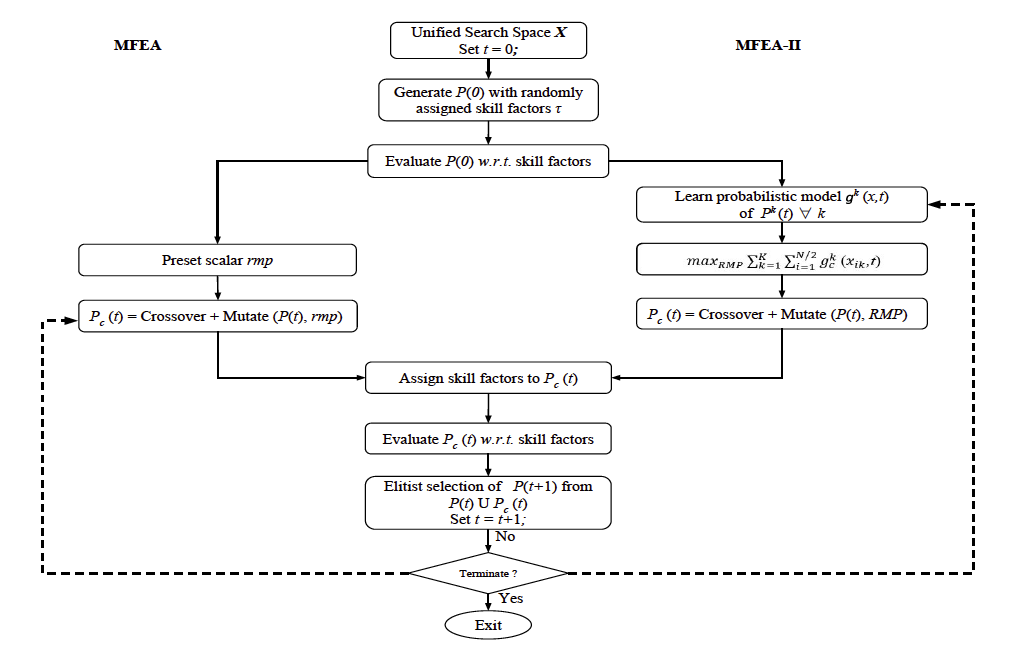
\includegraphics[width=1.0\linewidth, height=6.5cm]{images/mfeaii.png}
                    \caption{\small{MFEA-I và MFEAII}}
                    \label{fig:mfeaii}
                \end{figure}
        \end{columns}
	\end{frame}